\let\negmedspace\undefined
\let\negthickspace\undefined

\documentclass[journal,12pt,onecolumn]{IEEEtran}
%\documentclass[journal,12pt,twocolumn]{IEEEtran}
%
\usepackage{setspace}
\usepackage{gensymb}
%\doublespacing
\singlespacing

%\usepackage{graphicx}
%\usepackage{amssymb}
%\usepackage{relsize}
\usepackage[cmex10]{amsmath}
%\usepackage{amsthm}
%\interdisplaylinepenalty=2500
%\savesymbol{iint}
%\usepackage{txfonts}
%\restoresymbol{TXF}{iint}
%\usepackage{wasysym}
\usepackage{amsthm}
\usepackage{mathrsfs}
\usepackage{txfonts}
\usepackage{stfloats}
\usepackage{cite}
\usepackage{cases}
\usepackage{subfig}
%\usepackage{xtab}
\usepackage{longtable}
\usepackage{multirow}
%\usepackage{algorithm}
%\usepackage{algpseudocode}
\usepackage{enumitem}
\usepackage{mathtools}
\usepackage{tikz}
\usepackage{verbatim}
\usepackage{hyperref}
%\usepackage{stmaryrd}
\usepackage{tkz-euclide} % loads  TikZ and tkz-base
%\usetkzobj{all}
\usepackage{listings}
\usepackage{color}                                            %%
\usepackage{array}                                            %%
\usepackage{longtable}                                        %%
\usepackage{calc}                                             %%
\usepackage{multirow}                                         %%
\usepackage{hhline}                                           %%
\usepackage{ifthen}                                           %%
%optionally (for landscape tables embedded in another document): %%
\usepackage{lscape}     
\usepackage{multicol}
\usepackage{chngcntr}
\usepackage{iftex}
%\usepackage[latin9]{inputenc}
\usepackage{geometry}
\usepackage{bm}
%\geometry{verbose,tmargin=2cm,bmargin=3cm,lmargin=1.8cm,rmargin=1.5cm,headheight=2cm,headsep=2cm,footskip=3cm}
\usepackage{array}
\newcolumntype{L}[1]{>{\raggedright\let\newline\\\arraybackslash\hspace{0pt}}m{#1}}
\newcolumntype{C}[1]{>{\centering\let\newline\\\arraybackslash\hspace{0pt}}m{#1}}
\newcolumntype{R}[1]{>{\raggedleft\let\newline\\\arraybackslash\hspace{0pt}}m{#1}}

\usepackage{graphicx}
\usepackage{animate}
%\usepackage{setspace}
%\usepackage{parskip}

\def \hsp {\hspace{3mm}}

\makeatletter

\providecommand{\tabularnewline}{\\}



\makeatother
\ifxetex


%\DeclareUnicodeCharacter{03F5}{\ensuremath{\epsilon}}
%\DeclareUnicodeCharacter{03B3}{\ensuremath{\gamma}}
%\DeclareUnicodeCharacter{03B7}{\ensuremath{\eta}}
%\DeclareUnicodeCharacter{03C0}{\ensuremath{\pi}}
\usepackage{fontspec} 
\setmonofont{Liberation Sans} 
\usepackage{subfig}
%\setmainfont[ Path = fonts/]{Sanskrit_2003.ttf}
\usepackage{tikz}
\usepackage{xcolor}
%\usepackage{enumerate}

%\usepackage{wasysym}
%\newcounter{MYtempeqncnt}
\DeclareMathOperator*{\Res}{Res}
%\renewcommand{\baselinestretch}{2}
\renewcommand\thesection{\arabic{section}}
\renewcommand\thesubsection{\thesection.\arabic{subsection}}
\renewcommand\thesubsubsection{\thesubsection.\arabic{subsubsection}}

\renewcommand\thesectiondis{\arabic{section}}
\renewcommand\thesubsectiondis{\thesectiondis.\arabic{subsection}}
\renewcommand\thesubsubsectiondis{\thesubsectiondis.\arabic{subsubsection}}

% correct bad hyphenation here
\hyphenation{op-tical net-works semi-conduc-tor}
\def\inputGnumericTable{}                                 %%

\lstset{
	language=tex,
	frame=single, 
	breaklines=true,
	showstringspaces=false
}

%\begin{document}
%


\newtheorem{theorem}{Theorem}[section]
\newtheorem{problem}{Problem}
\newtheorem{proposition}{Proposition}[section]
\newtheorem{lemma}{Lemma}[section]
\newtheorem{corollary}[theorem]{Corollary}
\newtheorem{example}{Example}[section]
\newtheorem{definition}[problem]{Definition}
%\newtheorem{thm}{Theorem}[section] 
%\newtheorem{defn}[thm]{Definition}
%\newtheorem{algorithm}{Algorithm}[section]
%\newtheorem{cor}{Corollary}
\newcommand{\BEQA}{\begin{eqnarray}}
	\newcommand{\EEQA}{\end{eqnarray}}
\newcommand{\define}{\stackrel{\triangle}{=}}
\bibliographystyle{IEEEtran}
%\bibliographystyle{ieeetr}
\providecommand{\mbf}{\mathbf}
\providecommand{\pr}[1]{\ensuremath{\Pr\left(#1\right)}}
\providecommand{\qfunc}[1]{\ensuremath{Q\left(#1\right)}}
\providecommand{\sbrak}[1]{\ensuremath{{}\left[#1\right]}}
\providecommand{\lsbrak}[1]{\ensuremath{{}\left[#1\right.}}
\providecommand{\rsbrak}[1]{\ensuremath{{}\left.#1\right]}}
\providecommand{\brak}[1]{\ensuremath{\left(#1\right)}}
\providecommand{\lbrak}[1]{\ensuremath{\left(#1\right.}}
\providecommand{\rbrak}[1]{\ensuremath{\left.#1\right)}}
\providecommand{\cbrak}[1]{\ensuremath{\left\{#1\right\}}}
\providecommand{\lcbrak}[1]{\ensuremath{\left\{#1\right.}}
\providecommand{\rcbrak}[1]{\ensuremath{\left.#1\right\}}}
\theoremstyle{remark}
\newtheorem{rem}{Remark}
\newcommand{\sgn}{\mathop{\mathrm{sgn}}}
\providecommand{\abs}[1]{\left\vert#1\right\vert}
\providecommand{\res}[1]{\Res\displaylimits_{#1}} 
\providecommand{\norm}[1]{\left\lVert#1\right\rVert}
%\providecommand{\norm}[1]{\lVert#1\rVert}
\providecommand{\mtx}[1]{\mathbf{#1}}
\providecommand{\mean}[1]{E\left[ #1 \right]}
\providecommand{\fourier}{\overset{\mathcal{F}}{ \rightleftharpoons}}
%\providecommand{\hilbert}{\overset{\mathcal{H}}{ \rightleftharpoons}}
%\providecommand{\system}{\overset{\mathcal{H}}{ \longleftrightarrow}}
\providecommand{\system}[1]{\overset{\mathcal{#1}}{ \longleftrightarrow}}
\providecommand{\gauss}[2]{\mathcal{N}\ensuremath{\left(#1,#2\right)}}
%
%\newcommand{\solution}[2]{\textbf{Solution:}{#1}}
\newcommand{\solution}{\noindent \textbf{Solution: }}
\newcommand{\cosec}{\,\text{cosec}\,}
\newcommand{\sinc}{\,\text{sinc}\,}
\newcommand{\rect}{\,\text{rect}\,}
\providecommand{\dec}[2]{\ensuremath{\overset{#1}{\underset{#2}{\gtrless}}}}
\newcommand{\myvec}[1]{\ensuremath{\begin{pmatrix}#1\end{pmatrix}}}
\newcommand{\mydet}[1]{\ensuremath{\begin{vmatrix}#1\end{vmatrix}}}
\newcommand*{\permcomb}[4][0mu]{{{}^{#3}\mkern#1#2_{#4}}}
\newcommand*{\perm}[1][-3mu]{\permcomb[#1]{P}}
\newcommand*{\comb}[1][-1mu]{\permcomb[#1]{C}}
%\numberwithin{equation}{section}
\numberwithin{equation}{section}
%\numberwithin{problem}{section}
%\numberwithin{definition}{section}
\makeatletter
\@addtoreset{figure}{problem}
\makeatother
%\let\StandardTheFigure\thefigure
\let\vec\mathbf
%\renewcommand{\thefigure}{\theproblem.\arabic{figure}}
\renewcommand{\thefigure}{\arabic{section}.\arabic{figure}}
%\setlist[enumerate,1]{before=\renewcommand\theequation{\theenumi.\arabic{equation}}
	%\counterwithin{equation}{enumi}
	%\renewcommand{\theequation}{\arabic{subsection}.\arabic{equation}}
\let\StandardTheFigure\thefigure
	\vspace{3cm}
	%\usepackage{babel}
	\begin{document}
		\title{Learning Project On RL}
		\author{ Mannem Charan AI21BTECH11019}
		 \maketitle
		\begin{abstract}
		This report consists of my understanding on RL and different algorithms used to solve the RL problem and their implementation using Frozen-lake environment from OpenAI gym.
	       \end{abstract}

	       \tableofcontents

     \section{Introduction}
     Reinforcement Learning,is one way of machine learning where we try to design a \emph{learner} which can do the task at hand after learning.
       To understand it, first we will compare RL with other ways of learning,
       \begin{enumerate}

	       \item \textbf{Supervised Learning :} Here the model or learner \emph{learns} how to do the task under some \emph{supervision}.In other words, the model get to know the tags/\textit{labels} of the samples, using which it will try to predict the labels of the unseen data. \\
	\centerline{Examples\footnote{Here when we say examples we mean that these techniques use the learning mentioned to create an intelligent agent} : Linear Regression,SVM,etc} \\
	  So the key things are,
	       \begin{itemize}
		       \item The model or \textit{agent} gets immediate labels or \textit{rewards}, i.e., there is no delay in rewards. 
		       \item There is no exploration since agent learns from experience via training data.
	       \end{itemize}
       \item  \textbf{Un Supervised Learning :} Here the model learns how to do the task without any \emph{supervision}, that means here in training data we will not provide the
	labels. \\
	                     \centerline{Examples : K-means Clustering,DBSCAN,etc} \\
	  Here the key points are,
	        \begin{itemize}
			\item The model will not get any labels or rewards but it tries to learn the underlying pattern from the data(experience) given.
			\item There is no exploration since the experience that model gains only depends on training data.
		\end{itemize}

	\item	\textbf{Reinforcement Learning :} In Reinforcement Learning, we often use the term \textit{agent} for the learner and the place where the agent \textit{learns} is known as \textit{environment}.Here agent learns about the environment by making decisions i.e., decisions impart what agent learns. \\
		  So here the task is to make the agent learn the "good sequence of decisions" in the environment. And depending upon the decisions agent make, it will get reward and has some delayed consequences.So RL also takes future outcomes into consideration and tries to learn a good sequence of decisions which maximizes the total reward.\\
	The key points of RL which makes it differ from others are ,
	         \begin{itemize}
		     \item The agent will get rewards as it keeps learning i.e., there is no fixed rewards it depends on what decisions the agent make.
		     \item There will be exploration since agent learns about the world by interacting/exploring the world.
		 \end{itemize}
	\item \textbf{Terminology used in RL :} The following figure $\ref{env-agent}$ depicts how the agent interacts with environment.
	      \begin{figure}
		      \centering
		      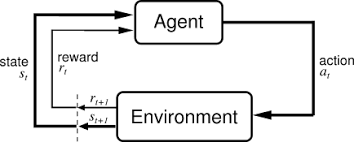
\includegraphics[width = 10cm]{Figs/action-state.png}
                      \caption{Agent and Environment}
		      \label{env-agent}
	      \end{figure}
	   \begin{enumerate}
		   \item Action $\brak{A}$ : All possible moves that agent can make on environment.Agent interact with environment with \emph{actions}. 
	     \item State $\brak{S}$ : State is the current position of agent returned by environment.
	     \item Reward $\brak{R}$ : The immediate return the agent gets from the environment to evaluate the last action.
	     \item Policy $\brak{\pi}$ :As the agent gains experience by making decisions/actions,it tries to design a map between the past experiences to the decisons or \textit{actions} to take.This is known as \textit{policy} $\brak{\pi}$. The goal of an agent is to find best or \textit{optimal}\footnote{To judge whether a policy is best or not we will evaluate the \emph{value} for the policy.Optimal policy is the one with maximum value.} policy for a given environment.
	     \item Value $\brak{V}$ : Contrast to reward, it is defined as the expected long-term return with discount $\brak{\gamma}$ \footnote{The factor used for penalising the future rewards.It is used to bound the \textit{value} of a state $\brak{\text{mathematical application}}$ but also have some importance in psychological sense.}when the agent is in certain state $s$ under a policy $\pi$. Mathematically we can write it as \footnote{This equation is also known as Bellman Equation which is the building block of RL},
		      \begin{align}
			      V^{\pi}\brak{s} = E\sbrak{R_{t+1} + \gamma V\brak{S_{t+1}} \vline S_{t} = s}
		      \end{align}
		      Here $t$ refers to the $t^{th}$ timestep.
	  \end{enumerate}
	\end{enumerate}
     With this terms in hand, we will now see explicitly how agent interacts with environment using OpenAI gym library.       
     \section{Environments using OpenAI Gym}
     Agent interact with the environment and learn from the experience.But often times it is hard to build the environment by hand when we begin learning the RL.The
     reward system should be designed carefully which helps the agent to understand what is the best way to make actions. \\ 
     Same as Imagenet, which made itself a benchmark for testing different ML techniques performance on the same training - testing data, there is something known as
     \href{https://www.gymlibrary.dev/}{Gym} which is used to test different RL algorithms. \\

In my project, I used "\href{https://www.gymlibrary.dev/environments/toy_text/frozen_lake/}{Frozen-Lake Environment}" a toy-text environment taken from Gym - a python library. Here is the code to be runned in terminal to get the gym library,
        \begin{lstlisting}
pip install gym==0.21.0
# New version has some bugs
	\end{lstlisting}
   Now after that, we can get our Frozen lake env with the following piece of code,
	\begin{lstlisting}[language = Python]
import gym

env = gym.make("FrozenLake-v1",desc= None,map_name = "8x8",is_slippery = False) 
env.reset() # Resets to current state.
env.render() # Used to show the current state of env.
#  S -> Start 
#  F -> Frozen Region
#  H -> Hole
#  G -> Goal
# Game starts at S and stops at H or G.And target is to reach G . 
       \end{lstlisting}
       The environment in the current state looks like \ref{ini_state1},
	      \begin{figure}
		      \centering
		      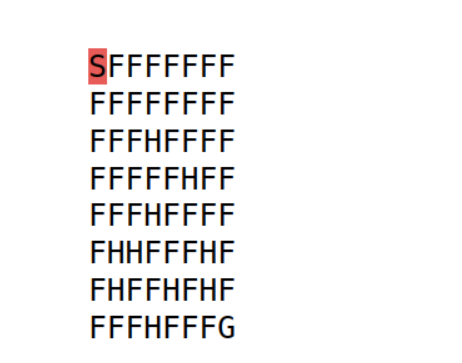
\includegraphics[width = 5cm]{Figs/cur_state1.png}
                      \caption{Initial State of Frozen Lake Environment}
		      \label{ini_state1}
	      \end{figure}
	      As the name itself self explanatory, the player will start at S and will move on Frozen regions F to reach goal G with minimum no.of steps without falling into the holes H.And the reward system looks like \footnote{It is different from the standard reward system mentioned in documentation, I changed that to visualise the performance of agents better}
        \begin{lstlisting}
Frozen (F) -> -0.01
Hole (H) -> -0.2
Goal (G) -> 1.0
       \end{lstlisting}
       The \textit{is\_slippery} attribute is used to make the frozen regions slippier so setting it to True or False changes the env according to that.I took both versions of environment and used different RL algorithms to obtain the optimal path.
        \section{Frozen Lake} 
	In this section, we will take default Frozen Lake environment without any slipperiness.To solve that, I used "\textbf{Q learning}" and "\textbf{SARSA}" algorithms to solve this RL problem.So we will see both of them one by one,
	\subsection{Solving using Q learning}
	  Similar to the value, Q-value is defined as the expected long-term reward with discount at given state $s$ and action $a$ under some policy $\pi$.
	  \begin{align}
		  Q^{\pi}\brak{s,a} &= E\sbrak{R_t + \gamma Q^{\pi}\brak{s',a'} \vline S_t = s , A_t = a}
	   \end{align}
	   In Q-learning, we will learn the Q-value for each state-action pair in iterative manner with optimal policy being greedy.So we will construct a state-action table where each pair has a Q-value as shown below,
       \begin{lstlisting}[language = Python]
State_space = env.observation_space
Action_space = env.action_space
Q = np.zeros((State_space.n,Action_space.n)) # Initialising with zeros.
           \end{lstlisting}
	   Then to interact with environment $\brak{\text{To explore}}$, we need a policy and I used $\epsilon$ - greedy algorithm to interact with the environment with $\epsilon$ being the probability to explore.You can see the code snippet below\footnote{The font used here is different in order to encode the unicode characters used here.}
	   \begin{verbatim}
def beh_policy(env,state,Q_table,ϵ):
 # explores with epsilon prob  
 if np.random.uniform() -ϵ < 1e-6:  
        return env.action_space.sample()
 else :
 # exploits with 1 - epsilon prob
        return np.argmax(Q_table[state])
	   \end{verbatim}
	   And as per Q learning we will update the Q value of each state-action pair $\brak{s,a}$ by following step, 
	     \begin{align}
		     Q\brak{s_t,a_t} \leftarrow Q\brak{s_t,a_t} + \eta\sbrak{\brak{r_t + \gamma max_{a}Q\brak{s_{t+1},a}} - Q\brak{s_t,a_t}}\label{Q_val_update}
	     \end{align}
                With $\eta$ being learning rate and $\gamma$ is discount factor. \\
		We can justify $\eqref{Q_val_update}$ as, we are updating the old Q value with the \emph{difference} of new Q-value \footnote{Q value obtained using greedy policy in the new state} and old Q-value under a learning rate $\eta$. As you can see it uses different policies to interact with env and to learn optimal policy.That's why Q learning algorithm also known as \textit{Off policy}. \\
		It is proven that, using Q learning algorithm with sufficient amount of training, one can find the \textit{ideal} next state for each state possible for the agent in the environment.So with that confidence I trained my agent for a \textit{total\_eps} $= 5000$ using the \textit{Q\_learning} function $\brak{\text{You can see the in FrozenLake.ipynb}}$. \\
      \textbf{Note :} In the code, I decreased $\epsilon$ as the agent trains because,in start I gave preference to \emph{explore} the environment,doing this helps agent to know about environment $\brak{\text{To know where the holes/frozen regions are}}$ and as it gained experience I allowed the agent to \emph{exploit} it's experience.\\

I used the following values for the hyperparameters and changing each value has its own kind of effect in the learning process.	Like if I decrease the $\epsilon$ 
or increase the $\epsilon_{min}$ it results in low performance of agent in training stage as it spends most of the time exploring. 
 \begin{verbatim}
η = 0.3 # Learning rate.

γ = 0.8 # Discount factor

ϵ = 0.9 # Prob to explore
ϵ_min = 0.1 # minimum epsilon as it decays.
π_Q,epi_list_Q,avg_time_step_Q,avg_rew_Q = Q_learning(env,η,γ,ϵ,ϵ_min,total_eps)
 \end{verbatim}
 As you can see the \textit{Q\_learning} returns,
     \begin{itemize}
      \item $\pi_Q \rightarrow$ The optimal policy designed by Q learning.
      \item $ epi\_list\_Q \rightarrow$ The list of episodes in which the agent reached the goal.
      \item $ avg\_time\_step\_Q \rightarrow$ The average time steps taken by the agent to reach the goal as it trains.
      \item $ avg\_rew\_Q \rightarrow$ The average reward recieved by the agent as it trains.
     \end{itemize}
Using these objects, we can see the performance of the agent in the training phase.
\subsection{Performance of Agent using Q learning}
 \begin{enumerate}
   \item \textbf{Success Rate :} Using $epi\_list\_Q$ we can determine no. of times agent reached the goal. 
 \begin{lstlisting}[language = Python]
print("Total no.of times agent reached the Goal in Training Phase {}".format(len(epi_list_Q)))
            \end{lstlisting}
            \begin{lstlisting}
Output -> Total no.of times agent reached the Goal in Training Phase 3896
            \end{lstlisting}
        In general this number twiddled around $3600$ to $4000$ which gives as the percentage of success being around 72 to 80.\\
	And the distribution of no.of times agent reached the goal as agent trained can be seen in fig \ref{epi-suc-Q},
	\begin{figure}[ht]
		      \centering
		      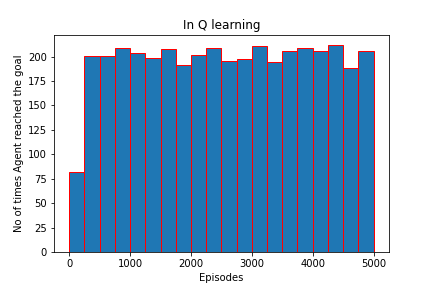
\includegraphics[width = 10cm]{Figs/hist_Q.png}
                      \caption{}
		      \label{epi-suc-Q}
	      \end{figure}

      \item \textbf{Average time steps taken :} You can see the Fig \ref{avg-time-Q},
	  \begin{figure}[ht]
		      \centering
		      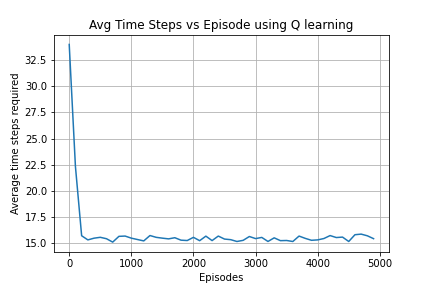
\includegraphics[width = 10cm]{Figs/Avg_time_Q.png}
                      \caption{}
		      \label{avg-time-Q}
	      \end{figure}
    Initially agent took more no.of time steps to reach the goal but after few hundred of episodes the average no.of time steps went down to around 15.
    And it became closer to 15 as it trained.\footnote{Eventhough the minimum no.of steps required to reach the goal is 14 since we are taking average of time steps for every $total_eps/50$ successfull episodes the value settled at 15.}
\item \textbf{Average reward gained :} You can see the fig \ref{avg-rew-Q}

	  \begin{figure}
		      \centering
		      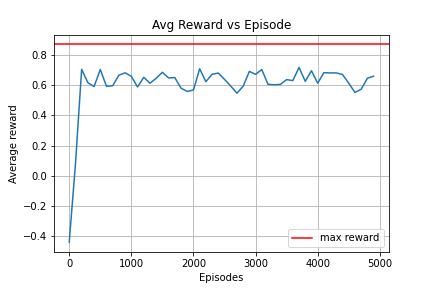
\includegraphics[width = 10cm]{Figs/Avg_rew_Q.png}
                      \caption{}
		      \label{avg-rew-Q}
	      \end{figure}

  From the figure we can interpret that, initially the agent recieved negative rewards most of the times.But as the training goes on it recieved positive rewards resulting in positive average rewards.In the end,it got an average reward of little over 0.6 and less than 0.7\footnote{Eventhough the maximum possible reward that agent can gain is $13 x -0.01 + 1 = 0.87$ the max average is below 0.8 since we are taking average of rewards recieved by agent}.
\item \textbf{Testing the optimal policy designed by Q learning :} Since the env is not slippery, the actions are not stochastic.This implies that,optimal policy should be able to reach the goal with minimum no.of steps.I used \textit{print\_frames} function to see the animation of agent reaching the goal with its optimal policy.
	    \begin{lstlisting}[language = Python]
from IPython.display import clear_output
from time import sleep

def print_frames(frames):
 for i, frame in enumerate(frames):
   clear_output(wait=True)
   print(frame['frame'])
   print(f"Timestep: {i + 1}")
   print(f"State: {frame['state']}")
   print(f"Action: {frame['action']}")
   print(f"Reward: {frame['reward']}")
  sleep(.2)
	 \end{lstlisting}
 I did one test run using the policy $\pi_{Q}$ because it is enough as actions are not stochastic.You can see the animation in the FrozenLake.ipynb file.\\
     The agent successfully learned the optimal path by taking only 14 steps to reach the goal,also received a maximum reward of 0.87.
       \end{enumerate}
    \subsection{Solving using SARSA}
    State-Action-Reward-State-Action \brak{SARSA} is an RL algorithm used to find the optimal policy for an agent traverse in the world. It is quite similar to \textbf{Q learning} other than the fact that SARSA is an \emph{on-policy}. It means that, it uses same policy to interact with environment as well as to estimate the optimal policy. So in place of the $\eqref{Q_val_update}$ we will use the following update step,
     \begin{align}
      Q\brak{s_t,a_t} \leftarrow Q\brak{s_t,a_t} + \eta\sbrak{\brak{r_t + \gamma Q\brak{s_ {t+1},a_{t+1}}} - Q\brak{s_t,a_t}}\label{Q_val_update_sarsa}
     \end{align}
     where the $s_t$ and $a_t$ are state and action taken using the policy at $t^{th}$ time step and $s_{t+1}$ is the next new state,$a_{t+1}$ is the next action to be taken using the same policy. Due to this sequential nature it is named as SARSA.\\
     Due to this difference in update step, the \textbf{performance} will vary in both algorithms.I will discuss the difference later but I implemented the SARSA algo using \text{SARSA} function $(\text{You can view the code in FrozenLake.ipynb file})$.\\
  And \textit{SARSA} function returns the same objects as \textit{Q\_learning} function.I trained the agent using \textit{SARSA} for 5000 episodes $\brak{\text{same as in Q learning}}$ and I took the same values for the $\eta, \gamma ,\cdots$ as I took for \textit{Q\_learning}. 	
  \begin{verbatim}
   total_eps = 5000 # Total no. of episodes to be trained

η = 0.3 # Learning rate.

γ = 0.8 # Discount factor

ϵ = 0.9 # Prob to explore
ϵ_min = 0.1 # minimum epsilon as it decays.

π_sarsa,epi_list_sarsa,avg_time_step_sarsa,avg_rew_sarsa = SARSA(env,η,γ,ϵ,ϵ_min,total_eps)
\end{verbatim}
 Similar to what we did in Q learning, we will understand how SARSA performed in training phase.
 \subsection{Performance of agent using SARSA}
   \begin{enumerate}
	
   \item \textbf{Success Rate :} Using $epi\_list\_sarsa$ we can determine no. of times agent reached the goal. 
\begin{lstlisting}[language = Python]
print("Total no.of times agent reached the Goal in Training Phase {}".format(len(epi_list_sarsa)))
            \end{lstlisting}
            \begin{lstlisting}
Output -> Total no.of times agent reached the Goal in Training Phase 4600
            \end{lstlisting}
	    In general this number twiddled around $4550$ to $4650$ which gives as the percentage of success being around 91 to 93.Whereas in case of Q learning, this is around 72 to 80.\\
       	    So clearly SARSA \textbf{outperformed} Q learning in terms of success rate in training. \\
	And the distribution of no.of times agent reached the goal as agent trained can be seen in fig $\ref{epi-suc-sarsa}$,
	\begin{figure}[ht]
		      \centering
		      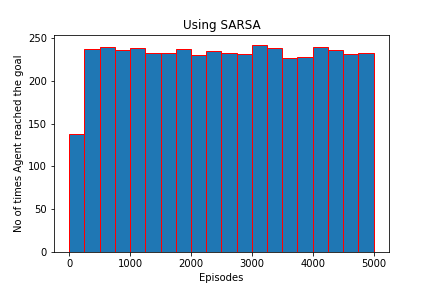
\includegraphics[width = 10cm]{Figs/hist_sarsa.png}
                      \caption{}
		      \label{epi-suc-sarsa}
	      \end{figure}
	 Here also in each \textit{bin}, the no .of episodes in which the agent reached the goal is higher compared to Q learning $(\text{compare with \ref{epi-suc-Q}})$. 
 \item \textbf{Average time steps taken :} You can see the plot in Fig \ref{avg-time-sarsa},

	 \begin{figure}[ht]
		      \centering
		      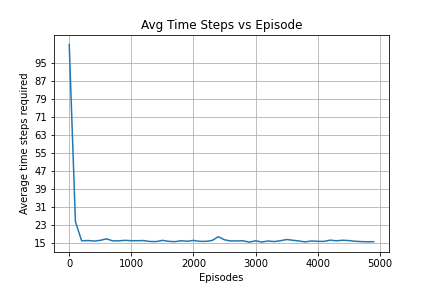
\includegraphics[width = 10cm]{Figs/Avg_time_sarsa.png}
                      \caption{}
		      \label{avg-time-sarsa}
	      \end{figure}
    As you can see initially agent took more no.of time steps to reach the goal but after few hundred of episodes the average no.of time steps went down to around 15.And it became closer to 15 as it trained.\\ 
    Compared to Q learning, even though the behaviour is same as it trains, initially SARSA took way more no.of steps to reach the goal compare to Q learning.   
\item \textbf{Average reward gained :} You can see the plot in fig \ref{avg-rew-sarsa}
	\begin{figure}[ht]
		      \centering
		      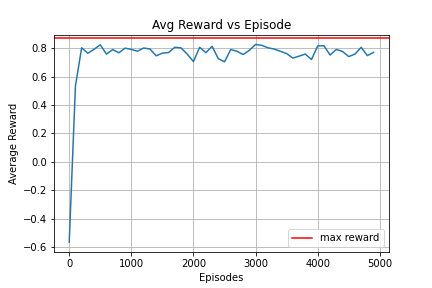
\includegraphics[width = 10cm]{Figs/Avg_rew_sarsa.png}
                      \caption{}
		      \label{avg-rew-sarsa}
	      \end{figure}

  From the figure we can interpret that, initially the agent recieved negative rewards most of the times.But as the training goes on it recieved more positive rewards resulting in positive average rewards.\\
  In the end,it got an average reward close to 0.87,which is the maximum possible reward.So in comparison with Q learning, SARSA has more negative avg rewards in early stages but as it trained it had \textbf{best} average reward compared to Q learning.
\item \textbf{Testing the optimal policy designed by SARSA :} Using the optimal policy $\pi_{sarsa}$ generated by SARSA, I did one test run $(\text{You can see the animation in FrozenLake.ipynb})$.\\
     And the agent reached the goal in minimum no.of steps of 14. So even though the \textbf{paths} taken by Q learning and SARSA are different they both reached the goal in same number of steps.\\
   \end{enumerate}
  \subsection{Q learning vs SARSA using custom map}
    So I wanted to know more about how the Q learning and SARSA \textbf{chooses} their paths,for which I changed the initial state of agent by giving custom map.You can do that by manually giving the initial map as shown below,
       \begin{lstlisting}[language = Python]
# Custom Env
env_cus = ["SFFFFFFF",
           "FFHHHHHF",
           "FFHFHFHF",
           "FFFHFFHF",
           "FFHFHFHF",
           "FFHFFHHF",
           "FHFFFFHF",
           "FFFHFFFG"]
env2 = gym.make("FrozenLake-v1",desc = env_cus,is_slippery = False)
env2.reset()
env2.render()
\end{lstlisting}
    The initial state looks like fig \ref{ini_state2}
    \begin{figure}[ht]
       \centering
       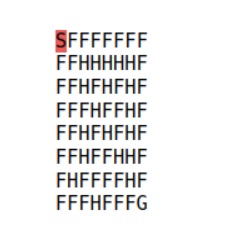
\includegraphics[width = 5cm]{Figs/cur_state2.png}
       \caption{}
       \label{ini_state2}
      \end{figure}
  \\ \textbf{Reason Behind using this custom env :}Since Q learning and SARSA are differ in their update step.I made this map, to see how Q learning and SARSA "choosing"  
 their paths.\\
 It is a \textbf{fact} that Q learning learns its \emph{optimal} path in less no.of steps. The reason behind this maybe because in its \emph{greediness} of choosing maximum Q value in the new state. So exploiting,in a way,is in the nature of Q learning. This tend to make the learning fast $(\text{taking less no.of time steps})$ after sufficient exploration. Whereas SARSA learns its \emph{optimal} path which is more \emph{safer} to reach the goal. Since the action selection is in it's nature,the SARSA tries to choose a path for agent which is more safer to reach the goal. So compare to Q learning it kinda explores more,which makes it to choose a safer path eventhough its a longer path $(\text{sometimes})$.\\
So in a way, Q learning tries to complete the task as soon as possible without thinking about safety of agent,whereas SARSA tries to choose a safe path to agent even though it costs more time to reach the goal.And depending on the application we should choose the appropriate algo. \\
So to \emph{check} these facts I designed this \ref{ini_state2} map which has 
       \begin{itemize}
	 \item A path of 14 steps by directly going 7 Right $(\rightarrow)$ steps and then by going 7 Down $(\downarrow)$ steps to reach Goal $(G)$.As you can see this path is surrounded by Holes $(H)$,so it can be considered as less safe path.
         \item A path of 16 steps by directly going 7 Down $(\downarrow)$ steps then 2 Right $(\rightarrow)$ steps, 1 Up $(\uparrow)$ step and going 2 Right $(\rightarrow)$ steps 1 Down $(\downarrow)$ step then going 2 Right $(\downarrow)$ steps. Compared to previous path it surrounded by less Holes $(H)$, so it can be considered as safe path though needing more steps to reach the goal.
       \end{itemize}
       \textbf{\underline{Observations after training}:}
       \begin{enumerate}
	       \item I trained the agent using the previous \textit{Q\_learning} function for the same \textit{total\_eps} of 5000 using the same values of $\eta,\gamma,\cdots$. And the agent it trained reached the goal in just 14 steps as we intended it to do. The performance in training phase can be seen below \footnote{You can refer FrozenLake.ipynb file for the plots},
	      
              \begin{figure}[ht]%
                \centering
		\subfloat[]{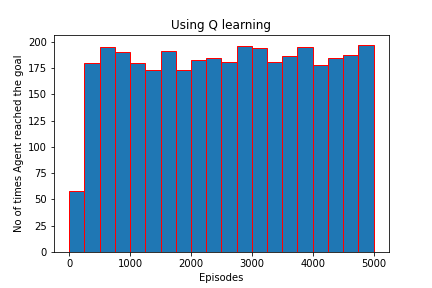
\includegraphics[width = 7cm]{Figs/hist2_Q.png}\label{fig:a}}%
		\subfloat[]{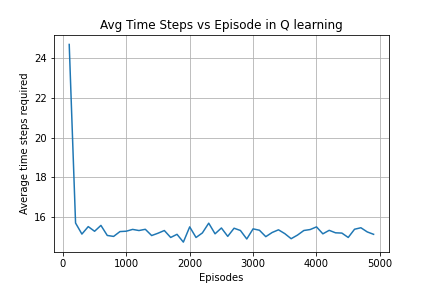
\includegraphics[width = 7cm]{Figs/Avg_time2_Q.png}\label{fig:b}}\\
		\subfloat[]{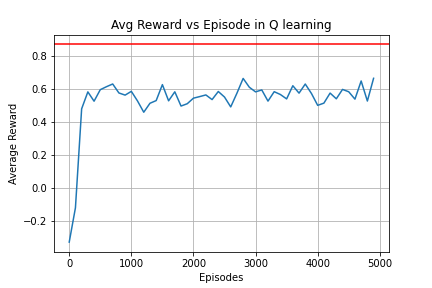
\includegraphics[width=7cm]{Figs/Avg_rew2_Q.png}\label{fig:c}}%
                \caption{Performance of agent trained with Q learning}%
                \label{Q learning}%
             \end{figure}

		
	\item Then I trained the agent using \textit{SARSA} for 5000 episodes but I failed to see any results. The agent actually not moving from the Start $(S)$,like it choosing Up $\brak{\uparrow}$ or Left $\brak{\leftarrow}$ as it's best actions.This behaviour can be reasoned as \emph{agent is fearing to move from Start position} i.e., it is thinking that staying there itself is the best course of action.So to make the agent reach the goal, I can do two things,
		          
		          \begin{itemize}
				  \item Increasing the no. of episodes to be trained which may help the agent to realise that there is a \textit{safer} path.
				  \item By changing the $\epsilon$ , $\epsilon_{min}$ values we can restrict the agent to exploit or explore more.
			  \end{itemize}
		  \item If I did the earlier way $\brak{\text{Call it SARSA-1}}$, the agent reached the goal in 16 steps everytime $\brak{\text{PS - I actually thought it will never happen}}$ after using a \textit{total\_eps} of $>=35000$ \footnote{ I tried different number of total eps but mostly the agent started reaching the goal using 35000 but then again I can't say this is the exact number}. \\ Here I did not changed the values of $\epsilon$ or $\epsilon_{min}$ so that, we can see that for the same \textit{degree of exploration} SARSA took around 35000 eps but Q learning took only 5000 eps to reach goal.You can see the plots for the perfomance of SARSA below,

	      \begin{figure}[ht]%
                \centering
		\subfloat[]{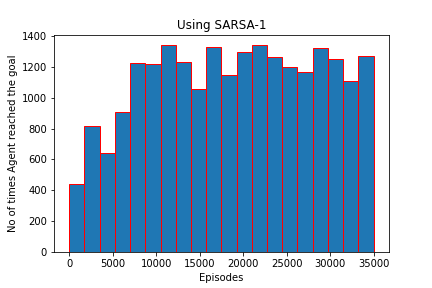
\includegraphics[width = 7cm]{Figs/hist2_sarsa1.png}\label{fig:a}}%
		\subfloat[]{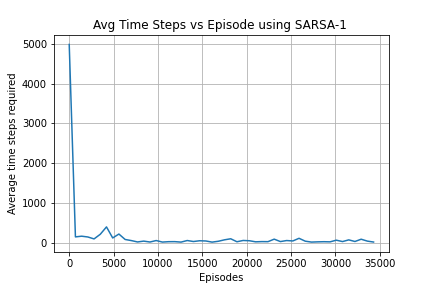
\includegraphics[width = 7cm]{Figs/Avg_time2_sarsa1.png}\label{fig:b}}\\
		\subfloat[]{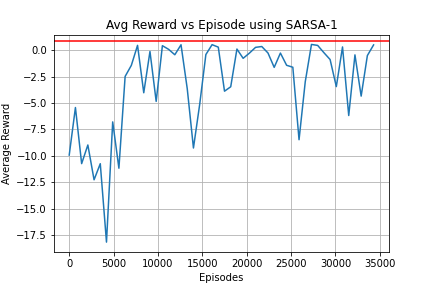
\includegraphics[width=7cm]{Figs/Avg_rew2_sarsa1.png}\label{fig:c}}%
                \caption{Performance of agent trained with SARSA-1}%
                \label{sarsa-1}%
             \end{figure}
		
     \item If I did the later way $\brak{\text{SARSA-2}}$, then suprisingly if I make $\epsilon = \epsilon_{min} = 0.1$ the agent reached the goal in 16 steps. I never saw this coming.And the performance in the training phase is irregular,i.e., sometimes it has good success rate in training phase and sometimes may not.But most of the time the end policy obtained can be used to reach the goal in 16 steps.It is not a good way to learn the path since most of the time we are exploiting instead of exploring the environment. I can't think of any specific reason but it maybe because it does not know that there is a path of 14 steps.With more degree of exploitation, the agent actions are more \textit{sensitive} to bad past experiences. So may be moving in Right $\brak{\rightarrow}$ from Start position must have gave agent bad experience which made it never move in that direction.You can see the plots to understand the performance of agent below, 
		 
	      \begin{figure}[ht]%
                \centering
		\subfloat[]{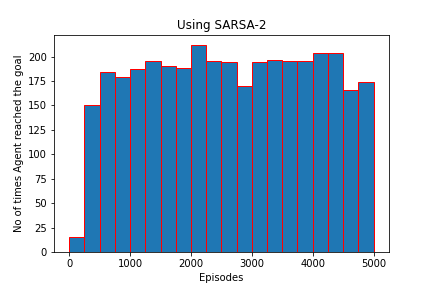
\includegraphics[width = 7cm]{Figs/hist2_sarsa2.png}\label{fig:a}}%
		\subfloat[]{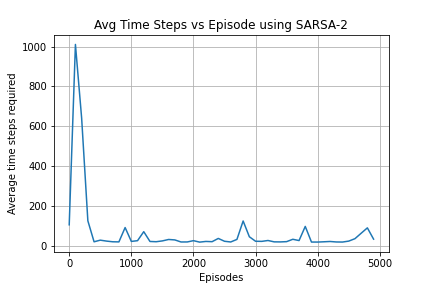
\includegraphics[width = 7cm]{Figs/Avg_time2_sarsa2.png}\label{fig:b}}\\
		\subfloat[]{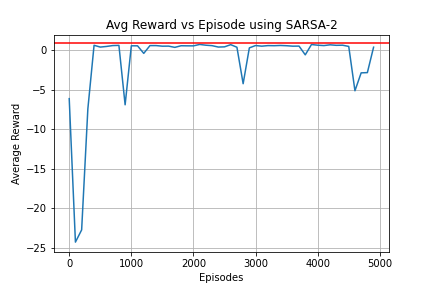
\includegraphics[width=7cm]{Figs/Avg_rew2_sarsa2.png}\label{fig:c}}%
                \caption{Performance of agent trained with SARSA-2}%
                \label{sarsa-2}%
             \end{figure}

	 \item Nonetheless both algos followed the intended behaviour when \textit{choosing} their optimal path.
	\end{enumerate}
    \textbf{Closing comments in Frozen Lake Env :}
      I used Q learning and SARSA algorithm to devise the optimal policy for the Frozen Lake Environment.Then I understood the difference of algorithms using a custom environment which is designed to know which \textit{optimal} path they took to reach the goal.

 \section{Frozen Lake with Slipperiness}
 In this section, I have taken the Frozen lake environment by setting $\textit{is\_slippery} = True$. So according to official documentation,the agent will move in intended direction with probability of $\frac{1}{3}$ else will move in either perpendicular direction with equal probability of $\frac{1}{3}$ in both directions. That is ,
    \begin{lstlisting}
For example, if action is left and is_slippery is True, then:
- P(move left)=1/3
- P(move up)=1/3
- P(move down)=1/3
    \end{lstlisting}
    So since, the actions are stochastic, one cannot find a \emph{deterministic} policy using which the agent can reach the goal everytime.So the \emph{optimal} policy here will be the one which has good success rate while testing the agent.\\
    To design the optimal policy I used the previously known Q learning and new algo known as \textit{Value Iteration}.\\
    \textbf{Value Iteration :} In value iteration, we will design the policy using the transition model of the environment.We will sweep through all the states and greedify them with respect to the current value function\footnote{ Value function is a function between state and it's \textit{value} but it generaly used as array with indexes being states}.After that we will design the policy by finding the best action to from the given which best maximises the value. You can see the below figure to understand better,  
    \begin{figure}[ht]
		\centering
		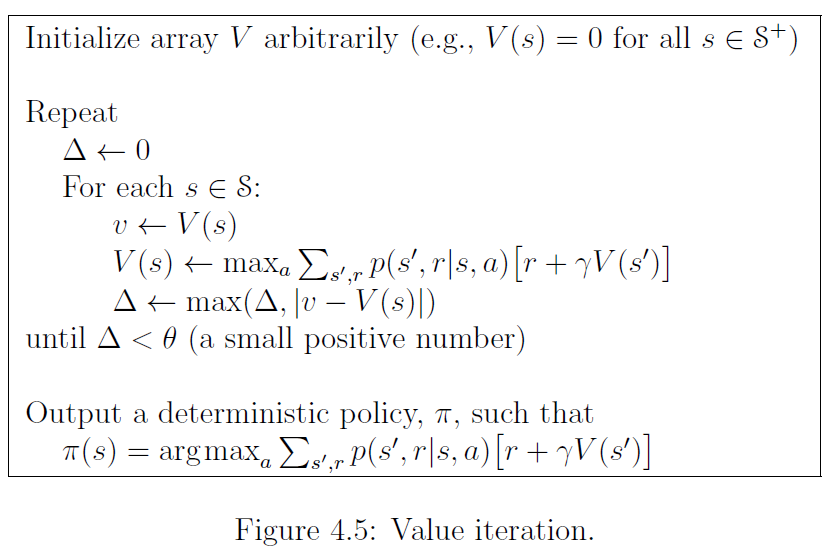
\includegraphics[width = 10cm]{Figs/val_ite.png}
		\caption{}
		\label{val-iter}
	\end{figure}
  \subsection{Perfomance of Q learning and Value Iteration}
    I trained one agent using Q learning for 5000 episodes and other agent using Value Iteration. Since actions are stocchastic, I tested both the agents for test\_eps using \textit{test\_ agent} function \footnote{You can refer the code}. You can see the difference in their performance with the plots below,
     \begin{enumerate}
	     \item \underline{Agent reaching the goal :} As you can see in Fig \ref{fig:1},agent trained with value iteration reached the goal more \textit{frequently} compared to agent trained with Q learning.
		     \begin{figure}[ht]%
                 \centering
                 \subfloat[\centering]{{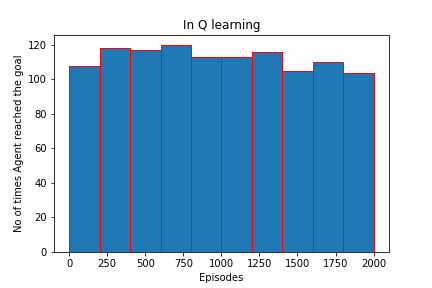
\includegraphics[width=5cm]{Figs/hist_Q_slippy.png} }}%
                 \qquad
                 \subfloat[\centering]{{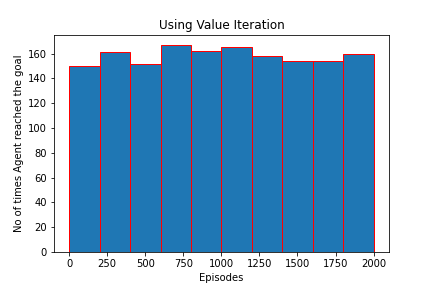
\includegraphics[width=5cm]{Figs/hist_val_slippy.png} }}%
                 \caption{Q learning vs Value Iteration in success rate.}%
                 \label{fig:1}%
                \end{figure}
	\item \underline{Average time taken :} As you can see in Fig \ref{fig:2}, the agent trained with value iteration in general took lesser \footnote{ Sometimes it happened that Q learning is on par with Value iteration but most of the times Value Iteration performed better than Q learning} no.of steps than Q learning.
                
		\begin{figure}[ht]%
                 \centering
                 \subfloat[\centering]{{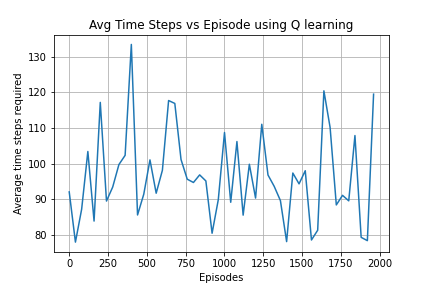
\includegraphics[width=5cm]{Figs/Avg_time_Q_slippy.png} }}%
                 \qquad
                 \subfloat[\centering]{{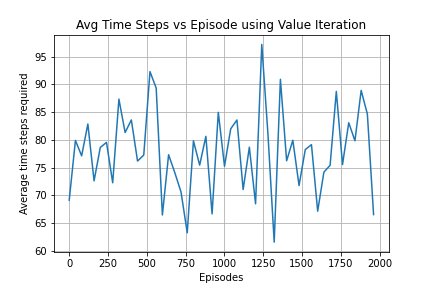
\includegraphics[width=5cm]{Figs/Avg_time_val_slippy.png} }}%
                 \caption{Q learning vs Value Iteration in average time taken}%
                 \label{fig:2}%
                \end{figure}
	\item \underline{Average reward gained :} As you can in Fig \ref{fig:3}, most of the times agent trained by Q learning recieved negative rewards whereas in case of Value iteration the agent recieved more positive rewards.
 
		\begin{figure}[ht]%
                 \centering
                 \subfloat[\centering]{{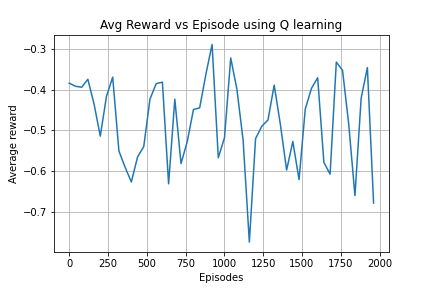
\includegraphics[width=5cm]{Figs/Avg_rew_Q_slippy.png} }}%
                 \qquad
                 \subfloat[\centering]{{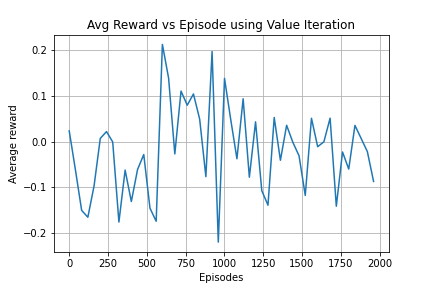
\includegraphics[width=5cm]{Figs/Avg_rew_val_slippy.png} }}%
                 \caption{Q learning vs Value Iteration in average reward gained}%
                 \label{fig:3}%
                \end{figure}
		So overall the agent trained by Value iteration gave better results than Q learning \footnote{Changing the no.of episodes to be trained in case of Q learning might improve the performance but after verifying many times the performance of Value Iteration is always better or on par with Q learning} 
        \end{enumerate}
  \section{Conclusion}
    \begin{itemize}
       \item In this report,I used Frozen Lake Environment to train the agent using different RL algorithms to achieve the optimal policy. 
       \item For the normal Frozen lake I used Q learning and SARSA algorithms to learn the optimal path. Both learned their own \textit{optimal} path to reach the goal. So to understand the way the both algos choose their paths I used a custom map which helped to reveal that Q learning learns the path with minimum no.of time steps whereas SARSA learns \textit{safer} path reach the goal.
       \item Then I took slippery version of Frozen Lake which motivated to use Value Iteration as it uses the transition model of the environment.I compared it with the old buddy Q learning by testing both algos for some no. of epsiodes. Then I observed that the agent trained with Value Iteration always performed better or on par with Q learning.
    \end{itemize}
       \end{document}
